\documentclass[titlepage]{article}
\usepackage[a4paper, total={6.5in, 8in}]{geometry}

\usepackage{preamble}

\title{
    \textbf{COMPARISON OF \\
    HEURISTIC ALGORITHMS \\
    FOR KP01} \\[0.5cm]
    \rule{12cm}{0.3mm} \\[0.5cm] 
    \small \scshape{A comparison of heuristic algorithms for solving the 0-1 Knapsack Problem} \\[0.4cm]
    \rule{12cm}{0.3mm}
    \vskip -0.3cm
}

\author{
    \small \scshape{Raunak Redkar} \\ 
    \small \scshape{Supervisors: Per-Olof Freerks and Felicia Dinnétz} \\
    \scriptsize \scshape{Kungsholmens Gymnasium}
}

\begin{document}


\renewcommand{\arraystretch}{1.5}

\onehalfspacing

\maketitle

\newpage

\begin{abstract}
    The 0-1 Knapsack problem is a well-known NP-complete problem. Various types of heuristic algorithms like genetic algorithms, simulated annealing algorithms, population evolution algorithms have been designed to solve the 0-1 Knapsack problem. The paper compared two such heuristic algorithms' ability to solve the 0-1 Knapsack Problem based on the generated total profit values: the BMQHOA (Binary Multi-Scale Harmonic Oscillator) Algorithm versus the DGHS (Discrete Global-Best Harmony Search) Algorithm. The algorithms were tested on 6 testgroups - 100, 1000, and 10000 randomized items, and uncorrelated, weakly correlated, and strongly-correlated items where the items are profit to weight correlated. The DGHS algorithm produced higher profit values on average than the BMQHOA algorithm in every testgroup. However, an unpaired t-test was performed and the difference in profit values produced between the two algorithms was evaluated as not statistically significant. The profit values produced by both algorithms in the uncorrelated, weakly-correlated, and strongly-correlated testgroups still showed the DGHS as superior, and the degree of correlation did not seem to have an affect on the profit values produced.  All codes for this paper are available at \href{github.com/raunakCode}{https://github.com/raunakCode/diploma-project}.
\end{abstract}

\newpage

\pagenumbering{roman}

\tableofcontents
\listofalgorithms
\newpage

\section{Introduction}

\pagenumbering{arabic}
\subsection{Background}

\renewcommand{\familydefault}{Computer Modern}
There are many situations in every day life, where people wonder whether they are doing something efficiently. Unforunately, the human brain is not always capable of coming up with an optimal approach when the problem has includes several factors to be accounted for. It is here when an external system is used, and the true power of computing can be recognised. 

To solve such problems, a computer is provided all the information, from which it will produce an optimal answer. For the system to process all the information, certain instructions must be written into the system so that it knows how to handle the information. This set of instructions is called an algorithm. The system or computer uses algorithms to take in information (the input), and produce an answer - the output. The efficiency (in all aspects) of the algorithm is dependant on the steps that make it up. Most problems have several algorithms which can solve them. For problems in computer science, more than one algorithm is usually proposed and used. This is usually the case for optimization problems. 

In the fields of computer science and mathematics, optimization problems are problems of finding the optimal solution, from a range of many feasible solutions. They are usually categorized into 2 categories: discrete optimizations and continuous optimizations, depending on whether the variables are discrete or continuous respectively. Combinatorial optimization problems are a subset of optimization problems that fall into the discrete. Combinatorial optimization involves searching for a maxima or minima for an objective function whose search space domain is discrete but usually large.

Typical combinatorial optimization problems include:
\begin{itemize}
    \item \textcolor{blue}{General Knapsack Problem} - Given a set of items, each with weight and profit value and a knapsack capacity, what is the best way to choose the items while respecting the knapsack capacity?
    \item \textcolor{blue}{Traveling Salesman Problem}- Given a list of cities, what is the shortest possible path that visits each city exactly once and returns to the origin?
    \item \textcolor{blue}{Set Cover} - Given a set of elements $\{1, 2, ..., n\}$ called the universe, and a collection of $m$ sets whose union equals the universe, what is the smallest sub-collection of those m sets whose union is the universe?
\end{itemize}

Combinatorial optimization problems show up in an array of different fields. The Knapsack Problem in particular has many variants which include the 0-1 knapsack problem, the bounded and unbounded knapsack problems, the multidimensional knapsack problem, the discounted knapsack problem, etc. The 0-1 Knapsack Problem is the simplest form of the knapsack problem and thus has also been in the main focus within the research community. It appears in real-world decision-making processes in a variety of fields. Some examples include: financial modelling and investments \cite{finance}, cryptography, and resource allocation in networking \cite{resource} (all considered high-scale instances of the knapsack problem; large amount of data to process).

Exact deterministic algorithms are those which will always produce the same optimal result every time. Many of combinatorial optimization problems including the 0-1 Knapsack problem currently do not have exact deterministic algorithms which are considered fast enough for them to be used in high-scale data situations. Consequently, the research focus has been on algorithms that do not necessarily guarantee the best solution but win over deterministic algorithms when it comes to time. 

\subsubsection*{Problem statement}
In the 0-1 Knapsack Problem, there are $n$ items and a maximum weight capacity $W$. Each item has a profit value $p_i$ and a weight value $w_i$. One must then find the optimal selection of items which maximizes the profit value while respecting the max weight value. The problem can be mathematically represented as such:

\vskip -0.5cm

\begin{gather}
    \text{Maximize}\;\; f(\Vec{x}) = \sum_{i = 1}^{n} p_i x_i \\
    \text{subject to} \sum_{i = 1}^{n} w_i x_i <= W \\
    x \in \{0, 1\}
\end{gather}

The rest of this paper will use the abbreviation "KP01" for the 0-1 Knapsack Problem. 

\subsection{Aim}
The aim of this paper is to compare the Discrete Global-Best Harmony Search Algorithm and the Binary Harmonic Multi-Scale Algorithm on their ability to solve KP01 to investigate the strength of the heuristic  techniques used for solving optimization problems.

\subsection{Research Question}
How do the Discrete Global-Best Harmony Search Algorithm and the Binary Harmonic Multi-Scale Algorithm perform when implemented for solving KP01?

\newpage

\section{Theory}
\subsection{Computational Complexity}
In computer science, computational complexity is the measure of how expensive it is to the run an algorithm; the amount of resources required to run the algorithm. The 2 resources are time and memory usage by a computer. As there are many low-level computer operations which happen, it is hard to exactly know how much time a program will take to run, however since these low-level operations always occur, the time taken for a program to run is usually some constant times some function of the size of the input - the time complexity. For this reason, the time and memory are usually given as time and space complexities which are given in terms of the size of the input.  As the memory complexity is dependent on the time complexity, the time complexity is the limiting factor for the efficiency of an algorithm and is usually the one focused on. Computable problems' time complexities can be factorial, exponential, polynomial, logarithmic, etc.

\subsubsection*{Big O notation}
The time complexity of an algorithm is a function of the size of the input of that algorithm. For example, if a set of $n$ numbers $a_1, a_2, a_3, ..., a_n$ are given, and an algorithm checks the existence of an certain number in that set, by checking all n elements of the set for equality, then the time complexity is some constant times $n$ - the size of the input. Computer scientists would denote this using Big O notation as $\mathcal{O}(n)$. Big O notation is a system developed by mathematicians and computer scientists to describe an function/algorithm's asymptotic limiting factor. \cite{bigO}

Computer scientists usually categories the time complexity of an algorithm into polynomial time complexities and non polynomial time complexities. This is because non-polynomial functions like factorial and exponential functions tend to grow quicker than polynomial functions and thus are usually considered nonviable for large data. One can see thus in the graph below before that the \textit{non-polynomial} functions like $f(x) = x!\cdot3^{x}$ or $f(x) = 2^{x}$ grow much faster than the other \textit{polynomial} or \textit{subpolynomial} functions. 

\vskip 1cm

% time complexities graph
\begin{center}
    \begin{tikzpicture}
      \begin{axis}[
          grid = major,
          clip = true,
          ticks = none,
          width=1\textwidth,
          height=0.8\textwidth,
          every axis plot/.append style={very thick},
          axis line style = ultra thick,
          clip mode=individual,
          restrict y to domain=0:10,
          restrict x to domain=0:10,
          axis x line = left,
          axis y line = left,
          domain = 0.00:10,
          xmin = 0,
          xmax = 11,
          ymin = 0,
          ymax = 11,
          xlabel = n,
          ylabel = Computer Operations,
          xlabel style = {at={(axis description cs:0.5,-0.1)},anchor=south},
          ylabel style = {at={(axis description cs:-0.08,0.5)},anchor=north},
          label style = {font=\LARGE\bf},
          ]
          \addplot [
            samples=100,
            color=red, 
          ] gnuplot{gamma(x+1)*3^x} node[above,pos=1,style={font=\Large}]{$\mathcal{O}(n!\cdot3^{n})$};
          \addplot [
            samples=100, 
            color=orange,
          ]
          {2^x}node[above,pos=1,style={font=\Large}]{$\mathcal{O}(2^{n})$};
          \addplot [
            samples=100, 
            color=green,
          ]
          {x}node[above,pos=1,style={font=\Large}]{$\mathcal{O}(n)$};
          \addplot [
            samples=100, 
            color=blue,
          ]
          {log2 x}node[above,pos=1,style={font=\Large}]{$\mathcal{O}(\log{}n)$};
          \addplot [
            samples=100,
            color=violet,
          ]
          {2*sqrt x}node[above,pos=1,style={font=\Large}]{$\mathcal{O}(2\sqrt{n})$};
          \addplot [
          samples=100, 
          color=red,
          ]
          {1}node[above,pos=1,style={font=\Large}]{$\mathcal{O}(1)$};
      \end{axis}
    \end{tikzpicture}
\end{center}

\subsubsection*{Complexity Classes}
All problems in computer science are classified into a complexity class, which describes how difficult it is to find a solution for the problem on demand \cite{complexity-class}. For example the class $P$ is is the set of problems which can be solved in polynomial time. The problems of the $NP$ class are those where a proposed solution to an instance of the problem can be verified in polynomial time, but a way of algorithmically determining an optimal solution in polynomial time is not (yet) known. $NP\text{-complete}$ problems are a subset of $NP$ problems for which it is possible to reduce any other problem in $NP$ to a problem in the subset $NP\text{-complete}$ in some polynomial time process. This is important, because then if it is then shown that the Knapsack Problem (an NP-complete problem) is actually in $P$ (a method of determining an optimal solution quickly exists), then all NP problems will be in $P$, proving $P=NP$, which is sometimes considered to be the most important problem in computer science \cite{PvsNP}. 

\textbf{Solving the 0-1 Knapsack Problem} \mbox{}\

There are 2 main approaches to solving KP01: An exact solution using deterministic algorithms, and probabilistic approaches involving heuristic algorithms. A small-scale KP01 can be solved with deterministic approaches, but for high-scale situations it is not realistic to get optimal solutions with exact approaches \cite{QWPA} as the KP01 problem is NP-complete \cite{KPNP}. 

\subsection*{Deterministic algorithms}
Dynamic programming is a general technique for solving optimization problems. If a problem has an optimal substructure and over-lapping subproblems, then dynamic programming is applicable . In computer science a problem has \emph{optimal substructure} if an optimal solution for a problem can be constructed from optimal solutions of its sub-problems, and \emph{over-lapping subproblems} is when a problem can be decomposed into sub-problems which are reused \cite{optimalSubstructure}. Dynamic programming breaks down a complicated problem into smaller sub-problems in a recursive manner, while also using some memory to save the solutions of the sub-problems (usually in tabular form). This way, when one needs to get a solution for a sub-problem again, one can just use previously calculated values. 

KP01 is solved using dynamic programming using a table based computation:

%dp
\begin{breakablealgorithm}
\caption{Solving 0-1 Knapsack with Dynamic Programming}\label{dp}
    \begin{algorithmic}[1]
        \For {$i = 0 \text{ to } noItems $} \Comment{\textcolor{blue}{If no items, then profit = 0}}
            \State $Table[i][0] \gets 0 $ 
        \EndFor
        \For {$k = 0 \text{ to } maxCapacity $} \Comment{\textcolor{blue}{If no capacity, then profit = 0}}
            \State $Table[0][k] \gets 0 $
        \EndFor
        \For {$i = 0 \text{ to } noItems$}
            \For {$k = 0 \text{ to } maxCapacity $}
                \State $Table[i][k] \gets Table[i-1][k]$  
                \If {$k-weights[i] >= 0$} 
                    \State $Table[i][k] \gets max(Table[i-1][k-weights[i]] + profits[i], Table[i][k]) $
                \EndIf
            \EndFor
        \EndFor
        \State $\textbf{Print } Table[noItems][maxCapacity] $
    \end{algorithmic}
\end{breakablealgorithm}

\vskip 0.5cm

This implementation of dynamic programming method has a time complexity of $\mathcal{O}(N\cdot W)$, where N is the number of items, and W is max capacity. The dynamic programming algorithm does not end until the entire table is built. This proves to be inefficient very quickly as the maximum capacity and the number of items in the knapsack increases. So, with the increase in the scale, the feasibility of dynamic programming decreases which has incentivized research in the subfield of heuristic algorithms \cite{QWPA}. 

\subsection*{Heuristic algorithms}
When deterministic algorithms prove to be too slow for practical applications such as online resource allocation, heuristic algorithms are chosen for their (usually) near optimal outputs and their speed. Heuristic algorithms should not be confused with approximation algorithms. Approximation algorithms guarantee a maximum margin of error; a constant factor off of the optimal. On the other hand, a heuristic algorithm does not guarantee anything, so it can perform better or worse than an approximation algorithm. 

Heuristic algorithms for combinatorial optimization are usually designed in a specific way \cite{heuristic}:
\begin{enumerate}
    \item Create a potential solution which is current best.
    \item Generate new solution. (usually in polynomial time) 
    \item If new solution better than current best, swap out the best with the newly generated. 
    \item If satisfied, output best solution, else continue.
\end{enumerate}

Both the Discrete Global-Best Harmony Search (DGHS), and Binary Multi-Scale Quantum Harmonic Oscillator (BMQHOA) have a similar framework.

\subsubsection{Discrete Global-Best Harmony Search Algorithm}
The Harmony Search algorithm (HS) was developed in 2001 based on the improvisation of music players who try to create better harmonies by adjusting previously known harmonies, hoping to produce more desirable ones \cite{geem01}. This algorithm was made for continuous search spaces and thus cannot be used for discrete search spaces in combinatorial optimization problems, as in KP01, items are either fully chosen or not, meaning one cannot add a fraction of the weight and the profit value of a particular item into the knapsack. The DGHS was proposed by Wan-li Xiang et al to overcome this by rounding decimals to the nearest integer value to discretize the search space \cite{DGHS-article}. The DGHS for KP01 also has a repair-operator and a greedy selection mechanism. A harmony in this algorithm refers to a candidate solution, or a certain selection of items to be put in the knapsack. 

It consists of 4 main parts:
\begin{enumerate}
    \item Create a harmony memory HM - a fixed size (HMS) of randomly generated harmonies. Initialize parameters harmony memory consider rate (HMCR), and pitch adjusting rate (PAR), and calculate profit-density vector for usage in the repair-operator.
    \item Create a new harmony using the current HM - Algorithm \ref{harmonyGen}.
    \item If generated harmony is better than the best in the harmony, replace it. If not, check if it is better than then worst harmony, and replace it if so. 
    \item If maximum number of iterations has been met, output the best sum profit value found so far.
\end{enumerate}

The 4 steps above take on the order of $nlogn$ time and thus have a time complexity of ${O}(n\log{}n)$.

\vskip 0.5cm
%DGHS
\begin{breakablealgorithm}
\caption{The DGHS algorithm}\label{DGHS}
    \begin{algorithmic}[1]
        \State Set the harmony memory size $HMS$, the number of iterations $ITERATIONS$, and the minimum and maximum values of parameters $PAR$ and $HMCR$.
        \State Initialize the HM through a randomized process, and use Algorithm \ref{harmonyRepair} to the generated harmonies. Calculate the totalProfit and totalWeight values for each harmony in HM.
        \State $iterator \gets 1$
        \While {$iterator <= ITERATIONS$}
            \State Record indices of the best and the worst harmonies in HM.
            \State Calculate parameters HMCR and PAR for the current iteration.
            \State Perform Algorithm \ref{harmonyGen} to produce a new harmony $\Vec{x}_{new}$
            \State Perform Algorithm \ref{harmonyRepair} to repair the new harmony $\Vec{x}_{new}$
            \If {$\Vec{x}_{new} \text{ is better than or equal to } \Vec{x}_{best}$}
                \State Replace $\Vec{x}_{best} \text{ with } \Vec{x}_{new}$
            \ElsIf {$\Vec{x}_{new} \text{ is better than or equal to } \Vec{x}_{worst}$}
                \State Replace $\Vec{x}_{worst} \text{ with } \Vec{x}_{new}$
            \EndIf
            \State $iterator \gets iterator+1$
        \EndWhile
        \State Output profit of best harmony
    \end{algorithmic}
\end{breakablealgorithm}
\vskip 0.5cm

The parameters HMCR and PAR are used when generating new harmonies. They determine the likelihood of heading toward the current best harmony, and the likelihood of randomly flipping a decision variable. The idea is that current best harmony should have an influence on the generation of a new harmony, and that a decision variable (whether or not an item is put in the knapsack) should be flipped to allow for diversity in the HM, making it easier to overcome local maxima. These parameters are determined in terms of the current iteration like so:

\begin{equation}
    HMCR(t) = HMCR_{max} - \frac{HMCR_{max}-HMCR_{min}}{ITERATIONS} t
\end{equation}
\begin{equation}
    PAR(t) = PAR_{max} - \frac{PAR_{max}-PAR_{min}}{ITERATIONS} t
\end{equation}

The dynamic updating of the parameters is designed in this way to let larger values of HMCR help accelerate the convergence of the harmonies early on with the the help of the best individual harmony, while smaller values of HMCR can help to overcome local maxima \cite{DGHS-article}. Similarly, larger values of PAR in the beginning allow for increases in diversity through mutations (item decision bit flips - deciding to take an item when having excluded it before or vice versa), when there is time to "explore" different variants, smaller values allow convergence at the end of the search. 


With these parameters one generates a new harmony:

%harmonyGen
\begin{breakablealgorithm}
\caption{Generating a new harmony during iterative part (part 2)}\label{harmonyGen}
    \begin{algorithmic}[1]
        \For {$i = 1 \text{ to } noItems$}
            \If {$rand(0, 1) <= HMCR(t)$}
                \State $newHarmony[i] \gets bestHarmony[i]$ 
            \Else
                \State Generate a random integer number $a \in \{1, 2, ... HMS\}, a \neq best$
                \State $newHarmony[i] \gets Harmony_{a}[i]$ 
                \If {$rand(0, 1) <= PAR(t)$}
                    \State $newHarmony[i] = |newHarmony[i]-1|$ \Comment{\textcolor{blue}{Flipping i'th item - mutation}}
                \EndIf
            \EndIf
        \EndFor
    \end{algorithmic}
\end{breakablealgorithm}
\vskip 0.5cm


Any time a harmony is generated, during Part 1 or Part 2, it is "repaired" in case the selection of items exceeds the capacity of the knapsack. The new generated harmony is also repaired if it can fit more items, without exceeding the capacity of the knapsack. The repair-operator consists of 2 phases:
\begin{enumerate}
    \item Drop phase - repairing a harmony if it violates the constraint
    \item Add phase - adding items into the knapsack if the new total weight is less than the capacity (the total weight of the knapsack stays below a previously decided value)
\end{enumerate}

The add phase is always done after the drop phase, as a harmony previously infeasible becomes feasible after the drop phase, but its total weight may be less than the capacity of the knapsack. Here is the pseudocode for the repair-operator:

\vskip 0.5cm
%harmonyRepair
\begin{breakablealgorithm}
\caption{Repair-operator for DGHS}\label{harmonyRepair}
    \begin{algorithmic}[1]
        \If {$totalWeight > maxWeight$}
            \For {$i = 1 \text{ to } N$} \Comment{\textcolor{blue}{DROP phase}}
                \State $\lambda_{i} = \frac{profit_{i}}{weight_{i}}$
            \EndFor
            \State Sort items in increasing order of $\lambda_{i}$, and let $ind_{i}$ denote the original index of each $\lambda_{i}$
            \For {$i = 1 \text{ to } noItems $} 
            \State Remove the ones with the least profit-density values greedily
                \If {$\lambda_{i} == 0$}
                    \State \textbf{Continue}
                \EndIf
                \State $newHarmony[ind_{i}] = 0$ \Comment{\textcolor{blue}{Unload the item}}
                \State $totalWeight \gets totalWeight - weight[ind_{i}]$
                \State $totalProfit \gets totalProfit - profit[ind_{i}]$
                \If {$totalWeight <= maxWeight$}
                    \State \textbf{Break} \Comment{\textcolor{blue}{Terminate DROP phase}}
                \EndIf
            \EndFor
        \EndIf
        \If {$totalWeight < maxWeight$}
            \For {$i = 1 \text{ to } N$} \Comment{\textcolor{blue}{ADD phase}}
                \State $\lambda_{i} = \frac{profit_{i}}{weight_{i}}$
            \EndFor
            \State Sort items in increasing order of $\lambda_{i}$, and let $ind_{i}$ denote the original index of each $\lambda_{i}$
            \For {$i = 1 \text{ to } noItems $} 
                \State Add the ones with the greatest profit-density if possible 
                \If {$newHarmony[ind_{i}] == 0$}
                    \If {$totalWeight + weight[ind_{i}] <= maxWeight$}
                        \State $newHarmony[ind_{i}] = 1$
                        \State $totalWeight \gets totalWeight + weight[ind_{i}]$
                        \State $totalProfit \gets totalProfit + profit[ind_{i}]$
                    \EndIf
                \EndIf
            \EndFor
        \EndIf
    \end{algorithmic}
\end{breakablealgorithm}

\vskip 1cm
\subsubsection{Binary Multi-Scale Quantum Harmonic Oscillator Algorithm}

The Multi-Scale Quantum Harmonic Oscillator Algorithm (MQHOA) is called as such as it follows a model of a solving a particle's ground state wave function under the harmonic oscillator potential well \cite{BMQHOA-article} . In MQHOA, candidate solutions are generated by sampling points in a Gaussian distribution within a certain distance of something. The Binary Multi-Scale Quantum Harmonic Oscillator Algorithm (BMQHOA) discretizes this by defining the number of bits between solutions (item decision variable) as the distance between solutions, so it becomes a discrete search space. Similar to the DGHS algorithm, a repair-operator is added to fix solutions that violate the capacity constraint. 

The BMQHOA algorithm consists of 4 parts:
\begin{enumerate}
    \item Random binary vector generation -> repair
    \item Generating a solutions by flipping $m$ items, mutating, and repairing
    \item Reducing the standard deviation value for the normal distribution from which the value for $m$ is determined during and for each iteration.
    \item If termination constraint is satisfied, output the best total profit value found so far, else return to Step 2.
\end{enumerate}

Similarly to the DGHS algorithm, the 4 steps above take on the order of $nlogn$ time and thus have a time complexity of ${O}(n\log{}n)$.

%BMQHOA
\begin{breakablealgorithm}
\caption{The BMQHOA algorithm with solution generation}\label{BMQHOA}
    \begin{algorithmic}[1]
        \State Set the number of iterations $ITERATIONS$ and the number of binary vectors (solutions) - BINVEC in memory.
        \State Randomly generate the binary vectors and use Algorithm \ref{harmonicRepair} to repair the vectors. 
        \While {$iterator <= ITERATIONS$}
            \State Update $\sigma_{s}$
            \State $found \gets FALSE$
            \While {$found == FALSE$}
                \State Try to generate a solution
                \State Let $solutions_{new}$ be the new generated vector 
                \State $solutions_{new} \gets solutions_{best}$
                \State Generate the number of flipped bits $m ~ N(0, \sigma_{s})$
                \State Treat $solutions_{new}$ as a circular array
                \State Randomly select a position in $solutions_{new}$ and flip the next $m$ items.
                \State Mutate a random bit towards current best solution (flip an item)
                \State $solutions_{new}[rand] \gets solutions_{best}[rand]$
                \State Repair newly generated solution
                \If {$totalProfit >= totalProfit_{worst}$}
                    \State Replace worst solution with newly generated solution
                    \State $solutions_{worst} \gets solutions_{new}$
                    \State $found = TRUE$
                \EndIf
            \EndWhile
        \EndWhile
    \end{algorithmic}
\end{breakablealgorithm}
\vskip 0.5cm

After generating a new solution, $m$ items are flipped in the aspiration of increasing diversity of the solutions and increasing the likelihood of finding the optimal solution. A normal distribution is defined by a mean value and a standard deviation. The value for $m$ is generated randomly by using a normal probability distribution which has a mean of $0$ and a Std. Deviation value which is determined by the iteration the algorithm is on. The Std. Deviation decreases with each new-solution-generation iteration so as to increase diversity in the beginning of the search, while reducing the likelihood of deteriorating a binary vector near the end of the search when close to optimal solutions have probably been found \cite{BMQHOA-article}. Initially the value of the standard deviation is set to $noItems/3$, so that there is a $\sim 99.7\%$ chance that the generated number of flipped items $m$ are in the range $[0-3\sigma_{s}, 0+3\sigma_{s}] \approx [-noItems, noItems]$, however in the case that $m \notin [-noItems, noItems]$, the value is reduced mod $noItems$:

$$STDEV_{max} = noItems/3$$
$$\sigma_{s} = 1-\frac{t}{ITERATIONS} STDEV_{max}$$

The normal distribution probability density function generator is implemented with the C++ Standard Library class normal\_distribution. An item's decision value is also made to match the corresponding decision in the best solution, which gives a slow mutation towards the current best solution allowing for diversity while still allowing the best solution to influence the process. This is because allowing multiple bits to mutate toward current best can lead to a premature local maximum, nullifying the rest of the search \cite{BMQHOA-article} . 

The repair-operator of the BMQHOA algorithm has 3 phases:
\begin{enumerate}
    \item Density-first stage: The already selected items are sorted based on their profit to weight ratio in non-increasing order and then greedily selected while respecting the weight constraint. 
    \item Minimum-weight-first stage: Out of the items that were not selected in the first stage are sorted based on their weight values in non-decreasing order, then greedily selected while respecting the weight constraint.   
\end{enumerate}

$Q_{1}[1, 2,...,n]$ is the index for the items in the density ratio array in the original vector. $Q_{2}[1, 2,..., n]$ is index of the items in the minimum weight sorted array in the original vector.

\begin{breakablealgorithm}
\caption{Repair-Operator for BMQHOA}\label{harmonicRepair}
    \begin{algorithmic}
        \State Let $x$ be the current array/vector.
        \State $totalWeight = 0, temp = 0, i = 0, b = 0$
        \State Stage 1: Density first stage
        \While {$temp < maxWeight$}
            \State $totalWeight = temp$
            \State $i += 1$
            \State $temp = temp + weight[Q_{1}[i]]$
        \EndWhile
        \For {$j = i \text{ to } n$}
            \State $x[Q_{1}[j]] = 0$
            \State $totalWeight += x[Q_{1}[j]]$
        \EndFor
        \State Stage 2: Minimum weight first stage
        \While {$totalWeight < C$}
            \State $b += 1$
            \If {$totalWeight + weight[Q_{2}[b]] <= C$} 
                    \State $x[Q_{2}[b]] = 1$
                \State $totalWeight += weight[Q_{2}[b]]$
            \EndIf
        \EndWhile
    \end{algorithmic}
\end{breakablealgorithm}

\newpage

\section{Methodology}

\subsection{Coding the algorithms}
The DP (dynamic programming) bruteforce was used to try all possible combinations of items to find the optimal profit value. The DP bruteforce algorithm, DGHS algorithm and the BMQHOA algorithm were coded in C++ based on the pseudocode provided in articles that proposed the respective algorithms. These C++ implementations of the algorithms can be found at \href{https://github.com/raunakCode/diploma-project/tree/main/algorithms}{\textcolor{blue}{https://github.com/raunakCode/diploma-project/tree/main/algorithms}}. 

\subsection{Generating testdata}
The testdata was categorized into 6 testgroups, each of which had 5 different testcases, each of which is an input on which every algorithm was run. 3 testgroups of 5 testcases were made using a random number generator, where a random number was generated using the Mersenne Prime Twister (mt19937) \cite{mersenne} with some C++ code - available \href{https://github.com/raunakCode/diploma-project/blob/main/testing/gen.cpp}{\textcolor{blue}{here}}. A computer cannot generate a truly random number. A pseudorandom number is what is generated, which is a number which appears to be statistically random, but has been generated using a deterministic process, in this case - the Mersenne Prime Twister. The 3 groups had item counts of 100, 1000, and 10000. The number of solutions in memory (for the heuristic algorithms) was put in the input file and was kept a constant, 20, in all testcases and algorithms for this report. 

In the 3 random number generated testgroups, the number of items $noItems$ was chosen to either be 100, 1000 or 10000. The profit and weight values were then randomly generated in a range of $ [1, noItems] $ while a sum-of-weights variable \emph{sum} was kept. The max weight was then randomly generated in a range of $[\frac{\text{sum}}{100} , \frac{\text{sum}}{10}]$, so that the knapsack would not be able to hold all the items. To avoid any integer overflow errors, all generated numbers and the sum of all the profit/weight values were kept below the max value of an \emph{int} which is $2^{31}-1$ in many programming languages.  Then $n$, $W$ (maxWeight), and each item (profit and weight values) were all put in an input file which was later used to test the algorithms. This process was repeated 6 times for each of 3 random-items testgroups.

The other 3 testgroups of 5 testcases were taken from a database \cite{dataset}. These 3 "testgroups" are mentioned/used several times in the literature for KP01. The 3 testgroups are uncorrelated, weakly correlated, and strongly correlated; the correlation being between the items' profit and weight values. The number of solutions in memory, 20, was added to each of these testcases as well. 

To make a fair comparison the number of $ITERATIONS$ (how many times a candidate solution is generated) was set to 100 for both algorithms. These input files were then saved for later testing of the algorithms. Each testcase was then run on each algorithm and raw data of the total profit values generated was then saved, refer to appendix.

\subsection{Testing}
The C++ codes were compiled with the GNU G++17 compiler. Every testcase in each testgroup was then tested 6 times on both algorithms, and the raw data (profit values generated) was then saved for further processing. An unpaired t-test was conducted over all the profit values for both algorithms respectively. Unpaired t-tests were also performed within each testgroup as well, however they the t-tests' evaluation of the data did not change and thus has not been shown here. 

\newpage

\section{Results}

\subsection{Raw Data}
Refer to the appendix for the \hyperlink{random100}{raw data} for the algorithms running on the six testgroups: 100, 1000, 10k randomized numbers respectively and 3 differently profit-weight correlated datasets. 
% \href{https://github.com/raunakCode/diploma-project/blob/main/testing/algorithms%20results.csv}{\textcolor{purple}{Link to results}}

\subsection{Processed Data}
The mean and standard deviations for each group can be viewed in the following corresponding tables and graphs:

\begin{changemargin}{8mm}{8mm} 
%100
\begin{table}[h!]
    \centering
    \scriptsize
    \caption{\scriptsize Shows the mean and StDev. of the total profit values produced in dataset of 100 randomized items} \label{100-mean}
    \begin{tabu}{|c|[1pt]c|c|c|c|c|c|}
        \tabucline[1pt]{1-6} 
        Testcase & 1 & 2 & 3 & 4 & 5 \\ [-1pt] \tabucline[1pt]{1-6} 
        DGHS Mean &4160.33$\pm$3.50 &2561$\pm$0 &5288$\pm$19.66 &3535$\pm$0 &1747$\pm$0 \\[1em] \hline
        Mean Percent deviation from optimal &0.21\%  &0\%  &0.40\%  &0\%  &0\%  \\ [-1pt] \tabucline[1pt]{1-6}
        BMQHOA Mean &3926.83$\pm$40.27 &2561.00$\pm$0 &4879$\pm$46.18 &3360.66$\pm$68.96 &1711.5$\pm$25.71 \\[1em] \hline
        Mean Percent deviation from optimal &5.80\% &0\%  &8.09\% &4.93\% &2.03\% \\ [-1pt] \tabucline[1pt]{1-6}
    \end{tabu}
\end{table}

\begin{figure}[hbt!]
    \centering
    \vspace{1em}
    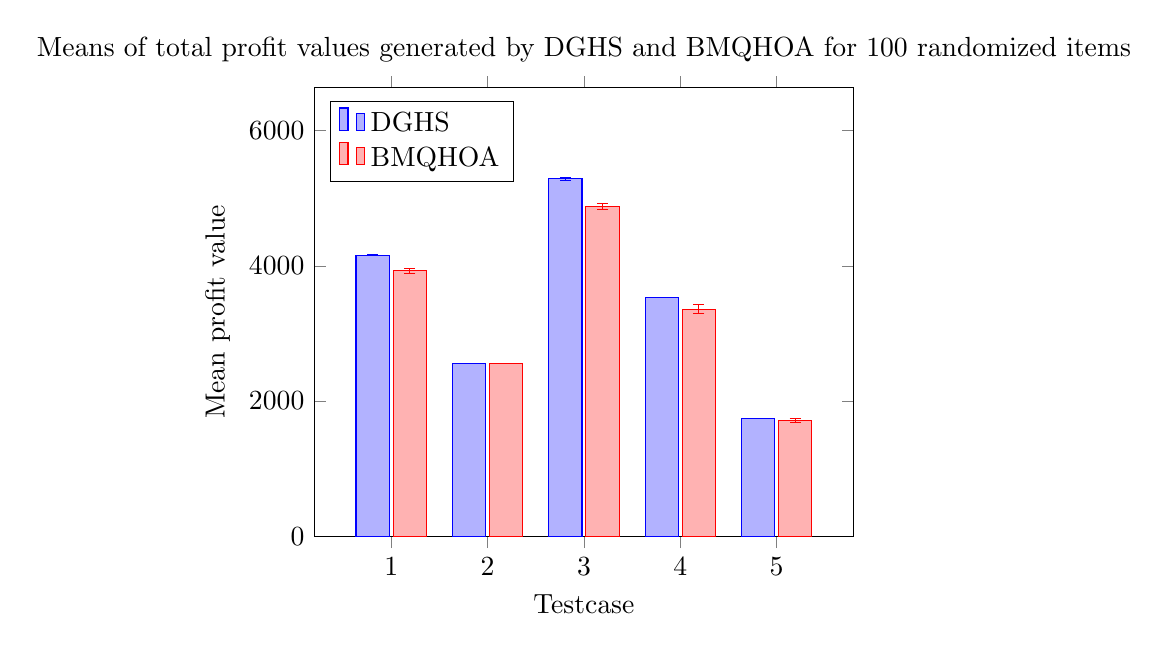
\begin{tikzpicture}
        \begin{axis} [
            title = Means of total profit values generated by DGHS and BMQHOA for 100 randomized items,
            ybar = .05cm,
            bar width = 12pt,
            xmin = 1,
            xmax = 5,
            ymin=0,
            xlabel = Testcase,
            ylabel = Mean profit value,
            legend cell align={left},
            legend pos = north west,
            %ytick = data,
            y tick label style={
            /pgf/number format/1000 sep=},
            enlarge y limits = {value = .25, upper},
            enlarge x limits = {abs = .8}
        ]
        \addplot+ [
                error bars/.cd,
                    y dir=both,
                    % (changed from `y explicit` so the error bars are (clearly) visible
                    y explicit ,
            ] coordinates {
                (1, 4160.33) +- (0,3.5)
                (2, 2561) +- (0,0)
                (3, 5288) +- (0,19.667)
                (4,3535) +- (0,0)
                (5,1747) +- (0,0)
            };
        \addplot+ [
                error bars/.cd,
                    y dir=both,
                    % (changed from `y explicit` so the error bars are (clearly) visible
                    y explicit ,
            ] coordinates {
                (1, 3926.83) +- (0,40.27613023)
                (2, 2561) +- (0,0)
                (3, 4879) +- (0,46.18224767)
                (4,3360.66) +- (0,68.9627919)
                (5,1711.5) +- (0,25.71186497)
            };
        \legend {DGHS, BMQHOA};
        \end{axis}
    \end{tikzpicture}
    \caption{Shows the means of profit values for 100 randomized items} \label{100-graph}
\end{figure}

%1000
\begin{table}
    \centering
    \scriptsize
    \caption{\scriptsize Shows the mean and StDev. of the total profit values produced in dataset of 1000 randomized items} \label{1000-mean}
    \begin{tabu}{|c|[1pt]c|c|c|c|c|c|}
        \tabucline[1pt]{1-6} 
        Testcase & 1 & 2 & 3 & 4 & 5 \\ [-1pt] \tabucline[1pt]{1-6} 
        DGHS Mean &156083.83$\pm$830.04 &118603.83$\pm$830.04 &144070$\pm$1343.77 &109734.33$\pm$1037.03 &126366.16$\pm$1236.73 \\ \hline
        Mean Percent deviation from optimal &13.71\% &11.76\% &14.12\% &10.77\% &13.27\% \\ [-1pt] \tabucline[1pt]{1-6}
        BMQHOA Mean &145086.5$\pm$1035.45 &109876.33$\pm$1540.63 &136622.66$\pm$2042.95 &101951.33$\pm$1271.88 &118291.16$\pm$799.78 \\ \hline
        Mean Percent deviation from optimal &19.79\% &18.25\% &18.56\% &17.10\% &18.82\% \\ [-1pt] \tabucline[1pt]{1-6}
    \end{tabu}
\end{table}

\begin{figure}[hbt!]
\centering
    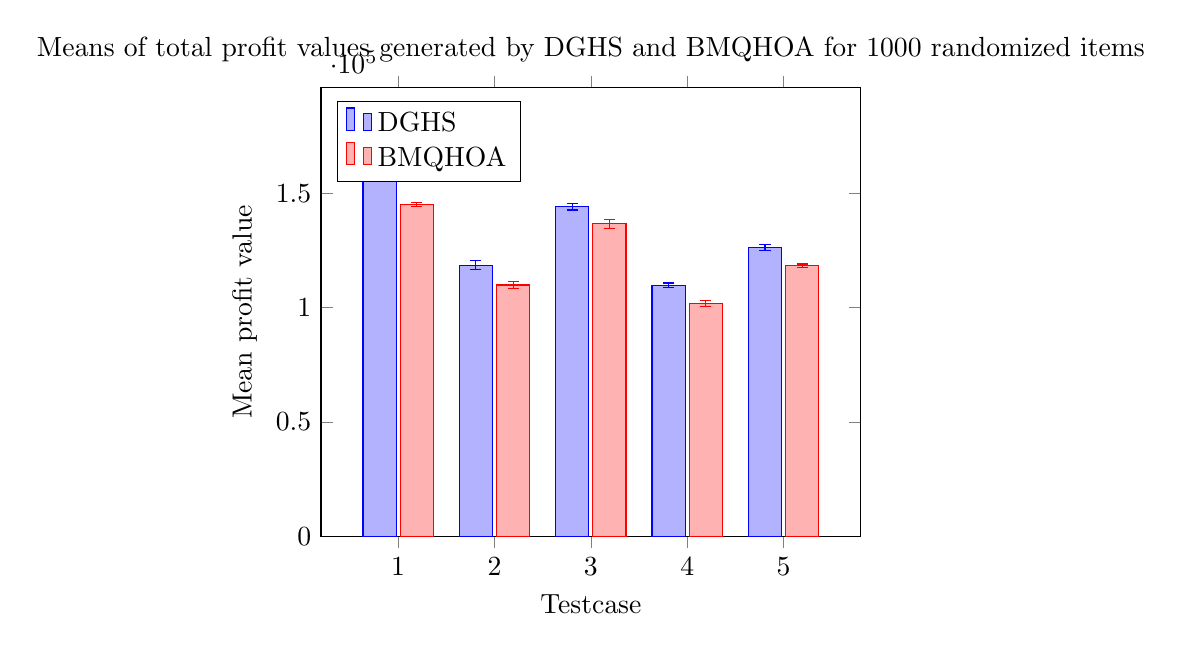
\begin{tikzpicture}
        \begin{axis} [
            title = {Means of total profit values generated by DGHS and BMQHOA for 1000 randomized items},
            ybar = .05cm,
            bar width = 12pt,
            xmin = 1,
            xmax = 5,
            ymin = 0,
            xlabel = Testcase,
            ylabel = Mean profit value,
            legend cell align={left},
            legend pos = north west,
            %ytick = data,
            y tick label style={
            /pgf/number format/1000 sep=},
            enlarge y limits = {value = .25, upper},
            enlarge x limits = {abs = .8}
        ]
        \addplot+ [
                error bars/.cd,
                    y dir=both,
                    % (changed from `y explicit` so the error bars are (clearly) visible
                    y explicit ,
            ] coordinates {
                (1, 156083.83) +- (0,830.04)
                (2, 118603.83) +- (0,1904.70)
                (3, 144070.00) +- (0,1343.77)
                (4, 109734.33) +- (0,1037.03)
                (5, 126366.17) +- (0,1236.73)
            };
        \addplot+ [
                error bars/.cd,
                    y dir=both,
                    % (changed from `y explicit` so the error bars are (clearly) visible
                    y explicit ,
            ] coordinates {
                (1, 145086.50) +- (0,1035.46)
                (2, 109876.33) +- (0,1540.63)
                (3, 136622.67) +- (0,2042.95)
                (4,101951.33) +- (0,1271.88)
                (5,118291.17) +- (0,799.79)
            };
        \legend {DGHS, BMQHOA};
        \end{axis}
    \end{tikzpicture}
\caption{Shows the means of profit values for 1000 randomized items} \label{1000-graph}
    \vspace{1em}
\end{figure}
\vskip -5cm
%10k
\begin{table}
    \centering
    \scriptsize
    \vspace{1cm}
    \caption{\scriptsize Shows the mean and StDev. of the total profit values produced in dataset of 10k randomized items} \label{10k-mean}
    \begin{tabu}{|c|[1pt]c|c|c|c|c|c|}
        \tabucline[1pt]{1-6} 
        Testcase & 1 & 2 & 3 & 4 & 5 \\ [-1pt] \tabucline[1pt]{1-6} 
        DGHS Mean &7681910$\pm$51555 &10567302$\pm$23956 &8014906$\pm$39449.15 &9347061$\pm$56967.66 &9583139$\pm$55816.60 \\ \hline
        Mean Percent deviation from optimal &22.61\% &23.11\% &22.07\% &23.10\% &23.00\% \\[-1pt] \tabucline[1pt]{1-6}
        BMQHOA Mean &7438487$\pm$29887.17 &10276681$\pm$50507.35 &7774520$\pm$34559.10 &9075476$\pm$53168.02 &9330322$\pm$46301.35 \\ \hline
        Mean Percent deviation from optimal &25.07\% &25.22\% &24.41\% &25.33\% &25.03\% \\[-1pt] \tabucline[1pt]{1-6}
    \end{tabu}
\end{table}

\begin{figure}[hbt!]
\centering
    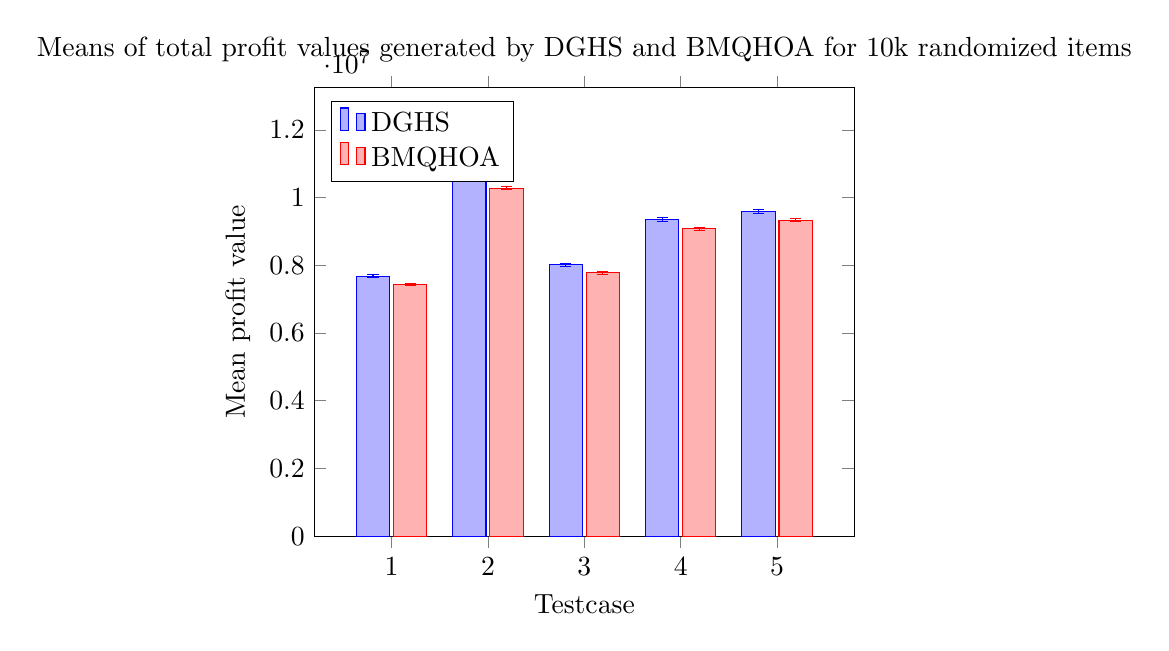
\begin{tikzpicture}
        \begin{axis} [
            title = Means of total profit values generated by DGHS and BMQHOA for 10k randomized items,
            ybar = .05cm,
            bar width = 12pt,
            xmin = 1,
            xmax = 5,
            ymin = 0,
            xlabel = Testcase,
            ylabel = Mean profit value,
            %ytick = data,
            legend cell align={left},
            legend pos = north west,
            y tick label style={
            /pgf/number format/1000 sep=},
            enlarge y limits = {value = .25, upper},
            enlarge x limits = {abs = .8}
        ]
        \addplot+ [
                error bars/.cd,
                    y dir=both,
                    % (changed from `y explicit` so the error bars are (clearly) visible
                    y explicit ,
            ] coordinates {
                (1, 7681910.333) +- (0, 51555.40)
                (2, 10567302) +- (0, 23956.32)
                (3, 8014906) +- (0, 39449.15)
                (4, 9347061.67) +- (0, 56967.67)
                (5, 9583139.17) +- (0, 55816.61)
            };
        \addplot+ [
                error bars/.cd,
                    y dir=both,
                    % (changed from `y explicit` so the error bars are (clearly) visible
                    y explicit ,
            ] coordinates {
                (1, 7438487.17) +- (0, 29887.18)
                (2, 10276681.83) +- (0, 50507.36)
                (3, 7774520.83) +- (0, 34559.11)
                (4, 9075476.00) +- (0, 53168.02)
                (5, 9330322.17) +- (0, 46301.35)
            };
        \legend {DGHS, BMQHOA};
        \end{axis}
    \end{tikzpicture}
\caption{Shows the mean of profit values for 10k randomized items} \label{10k-graph}
\end{figure}

%uncorrelated
\begin{table}[h!]
    \centering
    \scriptsize
    \caption{\scriptsize Shows the mean and StDev. of the total profit values produced in the profit-weight uncorrelated dataset} \label{uncorrelated-mean}
    \begin{tabu}{|c|[1pt]c|c|c|c|c|c|}
        \tabucline[1pt]{1-6} 
        Testcase & 1 & 2 & 3 & 4 & 5 \\ [-1pt] \tabucline[1pt]{1-6} 
        DGHS Mean &9147$\pm$0 &11238$\pm$0 &51019.50$\pm$437.85 &99036.16$\pm$1544.34 &448975$\pm$1135.46 \\ \hline
        Mean Percent deviation from optimal &0\% &0.00\% &6.39\% &10.47\% &20.34\% \\[-1pt] \tabucline[1pt]{1-6}
        BMQHOA Mean &8974.5$\pm$147.24 &10976.50$\pm$154.37 &47401.50$\pm$841.75 &91725.83$\pm$1346.23 &431259.66$\pm$3049.43 \\ \hline
        Mean Percent deviation from optimal &1.88\% &2.32\% &13.02\% &17.08\% &23.48\% \\[-1pt] \tabucline[1pt]{1-6}
    \end{tabu}
\end{table}

\begin{figure}[hbt!]
    \centering
    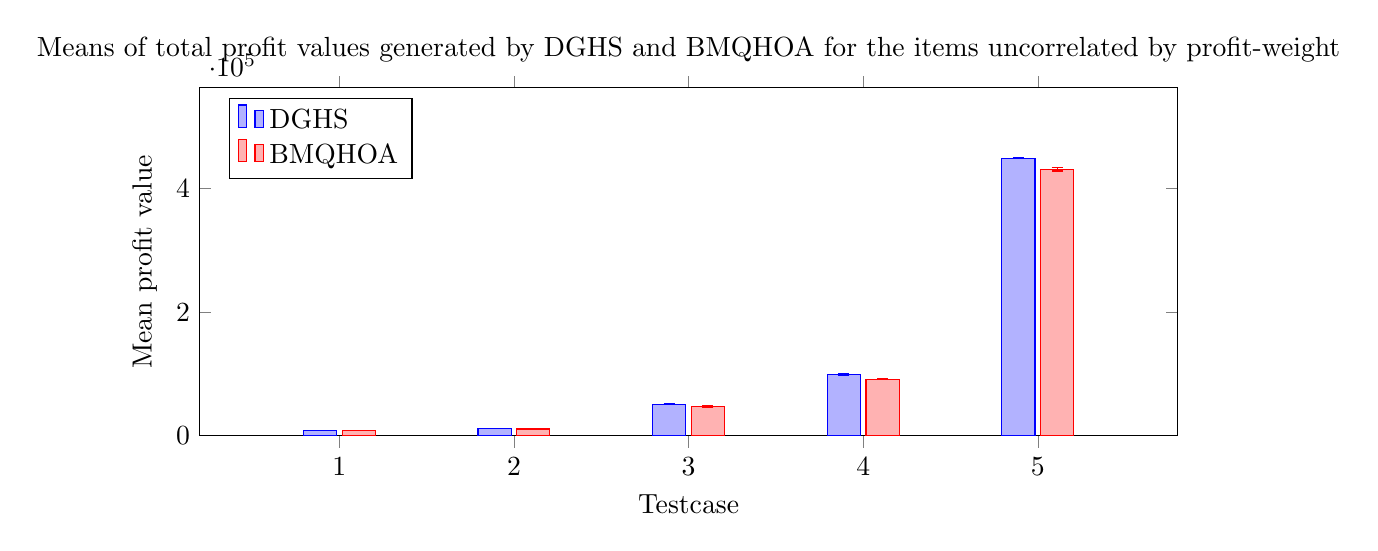
\begin{tikzpicture}
        \begin{axis} [
            title = Means of total profit values generated by DGHS and BMQHOA for the items uncorrelated by profit-weight,
            ybar,
            bar width = 12pt,
            width = 14cm,
            height = 6cm,
            xlabel = Testcase,
            ylabel = Mean profit value,
            xmin = 1,
            xmax = 5,
            ymin = 0,
            legend cell align={left},
            legend pos = north west,
            %x tick label style={rotate=45},
            xtick = data,
            ymin=0,
            %ytick = data,
            y tick label style={/pgf/number format/1000 sep=},
            enlarge y limits = {value = .25, upper},
            enlarge x limits = {abs = .8}
            %enlarge x limits = {abs = .8}
        ]
        \addplot+ [
                error bars/.cd,
                    y dir=both,
                    % (changed from `y explicit` so the error bars are (clearly) visible
                    y explicit ,
            ] coordinates {
                (1, 9147) +- (0, 0.00)
                (2, 11238.00) +- (0, 0.00)
                (3, 51019.50) +- (0, 437.85)
                (4, 99036.17) +- (0, 1544.34)
                (5, 448975.00) +- (0, 1135.46)
            };
        \addplot+ [
                error bars/.cd,
                    y dir=both,
                    % (changed from `y explicit` so the error bars are (clearly) visible
                    y explicit ,
            ] coordinates {
                (1, 8974.50) +- (0, 147.24)
                (2, 10976.50) +- (0, 154.37)
                (3, 47401.50) +- (0, 841.76)
                (4, 91725.83) +- (0, 1346.24)
                (5, 431259.67) +- (0, 3049.43)
            };
        \legend {DGHS, BMQHOA};
        \end{axis}
    \end{tikzpicture}
\caption{Shows the means of profit values for uncorrelated items} \label{uncorrelated-graph}
\end{figure}
\newpage
%weakly-correlated
\begin{table}[h!]
    \centering
    \scriptsize
    \caption{\scriptsize Shows the mean and StDev. of the total profit values produced in the profit-weight weakly-correlated dataset} \label{weakly-mean}
    \begin{tabu}{|c|[1pt]c|c|c|c|c|c|}
        \tabucline[1pt]{1-6} 
        Testcase & 1 & 2 & 3 & 4 & 5 \\ [-1pt] \tabucline[1pt]{1-6} 
        DGHS Mean &1514$\pm$0 &1627.66$\pm$2.42 &8907.33$\pm$27.56 &17371.83$\pm$126.76 &82681.33$\pm$390.98 \\ \hline
        Mean Percent deviation from optimal &0\% &0.38\% &1.59\% &3.76\% &8.33\% \\[-1pt] \tabucline[1pt]{1-6}
        BMQHOA Mean &1508.16$\pm$6.82 &1613.66$\pm$16.74 &8435.33$\pm$60.60 &16539$\pm$133.95 &80900.66$\pm$970.71 \\ \hline
        Mean Percent deviation from optimal &0.38\% &1.24\% &6.81\% &8.37\% &10.31\% \\[-1pt] \tabucline[1pt]{1-6}
    \end{tabu}
\end{table}

\begin{figure}[hbt!]
    %\centering
    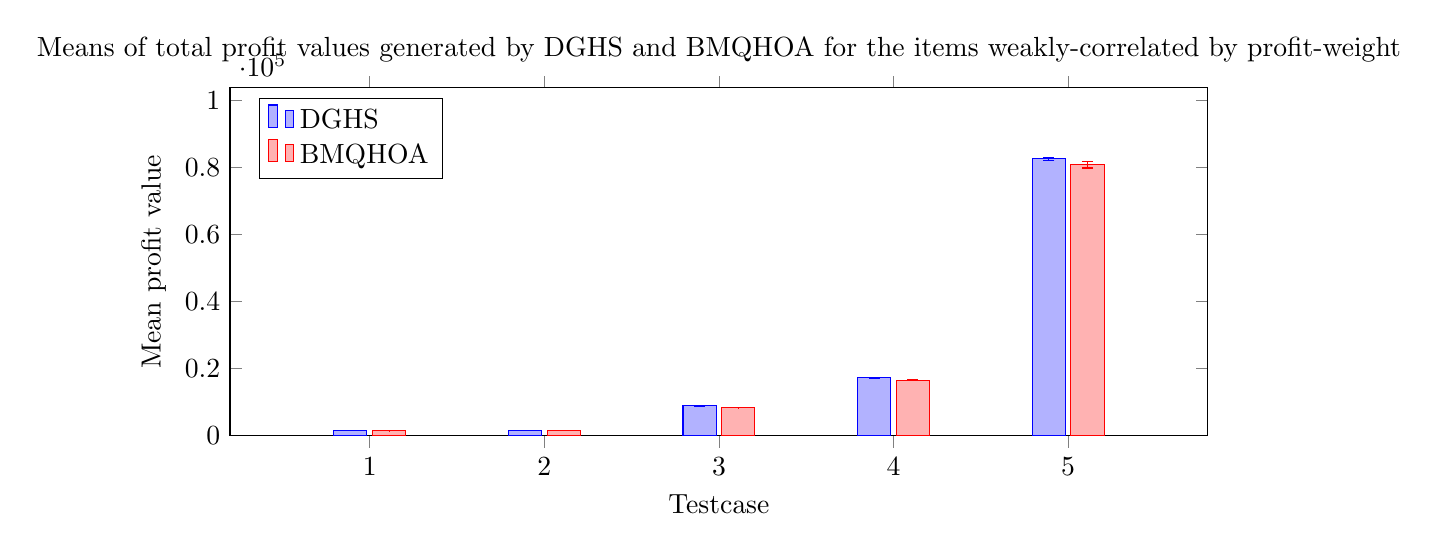
\begin{tikzpicture}
        \begin{axis} [
            title = Means of total profit values generated by DGHS and BMQHOA for the items weakly-correlated by profit-weight,
            ybar,
            bar width = 12pt,
            width = 14cm,
            height = 6cm,
            xlabel = Testcase,
            ylabel = Mean profit value,
            xmin = 1,
            xmax = 5,
            ymin=0,
            legend cell align={left},
            legend pos = north west,
            %x tick label style={rotate=45},
            xtick = data,
            %ytick = data,
            y tick label style={/pgf/number format/1000 sep=},
            enlarge y limits = {value = .25, upper},
            enlarge x limits = {abs = .8}
            %enlarge x limits = {abs = .8}
        ]
        \addplot+ [
                error bars/.cd,
                    y dir=both,
                    % (changed from `y explicit` so the error bars are (clearly) visible
                    y explicit ,
            ] coordinates {
                (1, 1514) +- (0, 0.00)
                (2, 1627.666667) +- (0, 2.422120283)
                (3, 8907.333333) +- (0, 27.56567914)
                (4, 17371.83333) +- (0, 126.7665834)
                (5, 82681.33333) +- (0, 390.9842282)
            };
        \addplot+ [
                error bars/.cd,
                    y dir=both,
                    % (changed from `y explicit` so the error bars are (clearly) visible
                    y explicit ,
            ] coordinates {
                (1, 1508.166667) +- (0, 6.823977335)
                (2, 1613.666667) +- (0, 16.74116683)
                (3, 8435.333333) +- (0, 60.6025302)
                (4, 16539) +- (0, 133.9596954)
                (5, 80900.66667) +- (0, 970.7196643)
            };
        \legend {DGHS, BMQHOA};
        \end{axis}
    \end{tikzpicture}
\caption{Shows the means of profit values for weakly correlated items} \label{weakly-graph}
\end{figure}


%strongly correlated
\begin{table}[h!]
    \centering
    \scriptsize
    \caption{\scriptsize Shows the mean and StDev. of the total profit values produced in the profit-weight strongly-correlated dataset} \label{strongly-mean}
    \begin{tabu}{|c|[1pt]c|c|c|c|c|c|}
        \tabucline[1pt]{1-6} 
        Testcase & 1 & 2 & 3 & 4 & 5 \\ [-1pt] \tabucline[1pt]{1-6} 
        DGHS Mean &2391.66$\pm$6.08 &2697$\pm$0 &13682.5$\pm$60.05 &26444.66$\pm$240.84 &126448$\pm$615.61 \\ \hline
        Mean Percent deviation from optimal &0.22\% &0\% &4.91\% &8.55\% &13.93\% \\[-1pt] \tabucline[1pt]{1-6}
        BMQHOA Mean &2327.33$\pm$48.55 &2658.66$\pm$48.81 &13334.66$\pm$182.91 &25604$\pm$91.32 &123813.83$\pm$773.19 \\ \hline
        Mean Percent deviation from optimal &2.90\% &1.42\% &7.33\% &11.46\% &15.72\% \\[-1pt] \tabucline[1pt]{1-6}
    \end{tabu}
\end{table}

\begin{figure}[hbt!]
    %\centering
    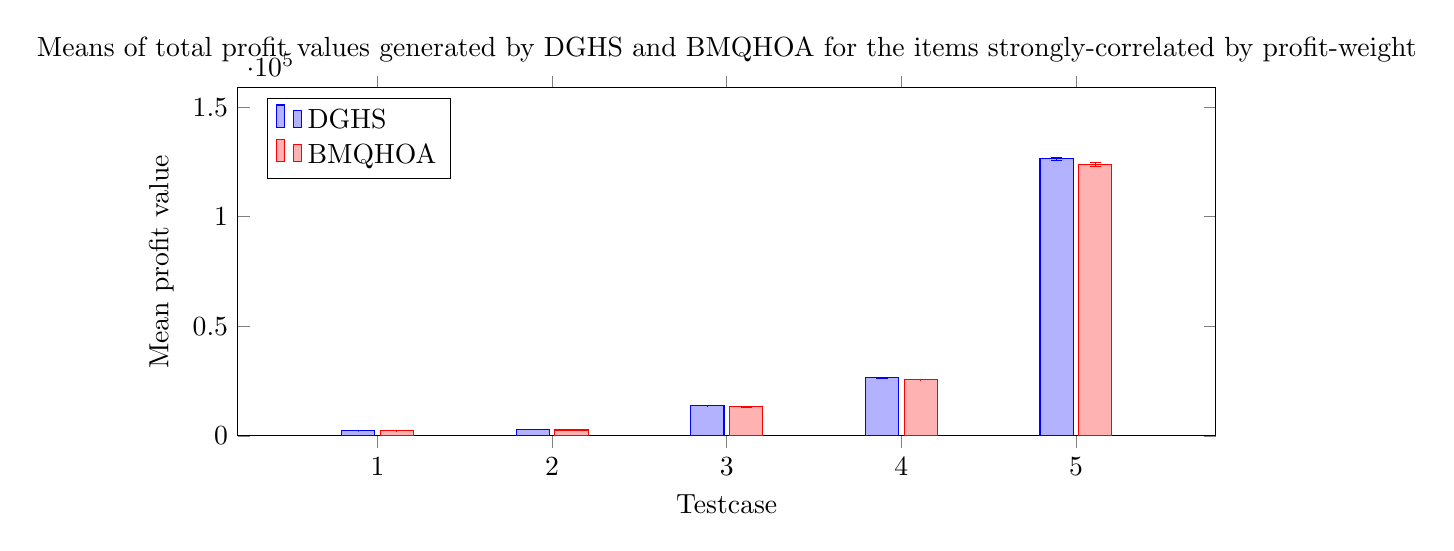
\begin{tikzpicture}
        \begin{axis} [
            title = Means of total profit values generated by DGHS and BMQHOA for the items strongly-correlated by profit-weight,
            ybar,
            bar width = 12pt,
            xlabel = Testcase,
            ylabel = Mean profit value,
            width = 14cm,
            height = 6cm,
            xmin = 1,
            xmax = 5,
            ymin = 0,
            legend cell align={left},
            legend pos = north west,
            %x tick label style={rotate=45},
            xtick = data,
            %ytick = data,
            y tick label style={/pgf/number format/1000 sep=},
            enlarge y limits = {value = .25, upper},
            enlarge x limits = {abs = .8}
            %enlarge x limits = {abs = .8}
        ]
        \addplot+ [
                error bars/.cd,
                    y dir=both,
                    % (changed from `y explicit` so the error bars are (clearly) visible
                    y explicit ,
            ] coordinates {
                (1, 2391.666667) +- (0, 6.08824003)
                (2, 2697) +- (0, 0)
                (3, 13682.5) +- (0, 60.05580738)
                (4, 26444.66667) +- (0, 240.8407496)
                (5, 126448) +- (0, 615.61384)
            };
        \addplot+ [
                error bars/.cd,
                    y dir=both,
                    % (changed from `y explicit` so the error bars are (clearly) visible
                    y explicit ,
            ] coordinates {
                (1, 2327.333333) +- (0, 48.55375028)
                (2, 2658.666667) +- (0, 48.81666382)
                (3, 13334.66667) +- (0, 182.9160099)
                (4, 25604) +- (0, 91.32579044)
                (5, 123813.8333) +- (0, 773.1955553)
            };
        \legend {DGHS, BMQHOA};
        \end{axis}
    \end{tikzpicture}
\caption{Shows the means of profit values for strongly correlated items} \label{strongly-graph}
\end{figure}

%mean percentage deviation
\begin{table}[h!]
    \centering
    \scriptsize
    \caption{\scriptsize Shows the mean percentage deviation from optimal total profit value across all datasets}\label{deviation-table}
    \begin{tabu}{|c|c|c|}
        \tabucline[1pt]{1-6} 
        & DGHS mean percentage deviation & BMQHOA mean percentage deviation \\ [-1pt] \tabucline[1pt]{1-6} 
        100 randomized items &0.12\% &4.17\% \\ \hline
        1000 randomized items &12.73\%&18.50\% \\\hline
        10k randomized items &22.78\%&25.01\% \\\hline
        Uncorrelated dataset &7.44\%&11.56\% \\\hline
        Weakly Correlated dataset &2.81\%&5.42\% \\\hline
        Strongly Correlated Dataset &5.52\%&7.77\% \\[-1pt] \tabucline[1pt]{1-6} 
    \end{tabu}
\end{table}

\begin{figure}[hbt!]
\centering
    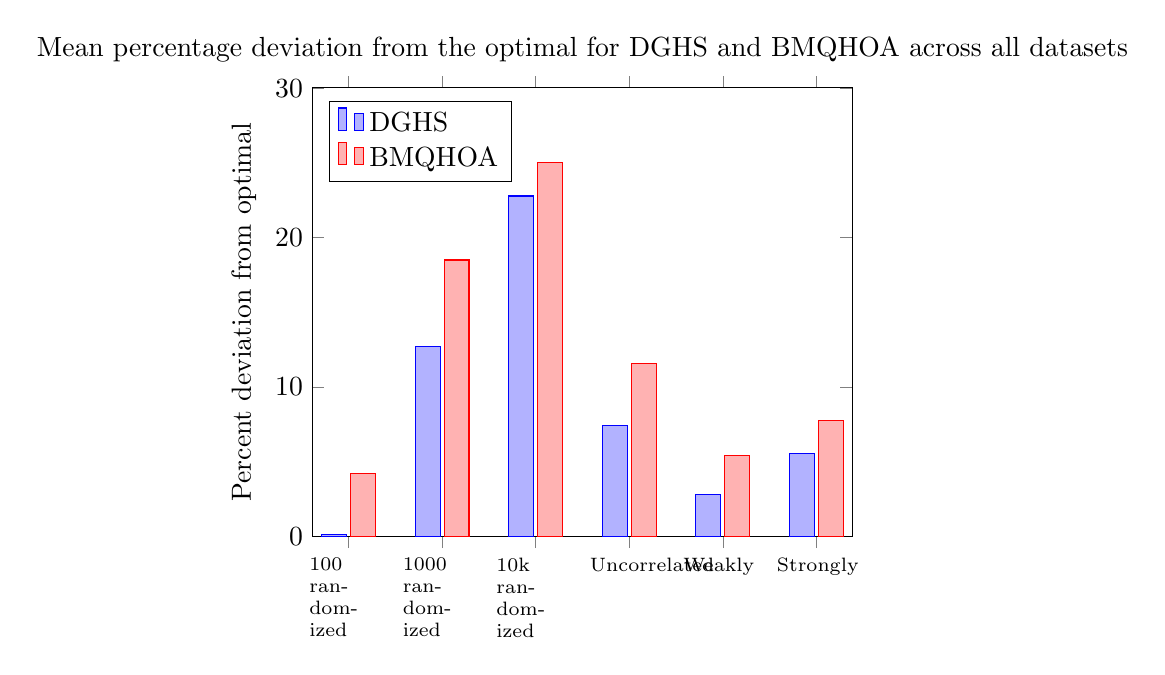
\begin{tikzpicture}
        \begin{axis} [
            title = {Mean percentage deviation from the optimal for DGHS and BMQHOA across all datasets},
            ybar = .05cm,
            bar width = 9pt,
            symbolic x coords={100 randomized, 1000 randomized, 10k randomized, Uncorrelated, Weakly, Strongly},
            x tick label style={font=\scriptsize,text width=1cm,align=left},
            ymin=0,
            ylabel = Percent deviation from optimal, 
            legend cell align={left},
            legend pos = north west,
            %ytick = data,+
            enlarge y limits = {value = .2, upper},
            enlarge x limits = {abs = 13pt}
        ]
        \addplot+[] coordinates {
            (100 randomized, 0.12)
            (1000 randomized, 12.73)
            (10k randomized, 22.78)
            (Uncorrelated, 7.44)
            (Weakly, 2.81)
            (Strongly, 5.52)
        };
        \addplot+[] coordinates {
            (100 randomized, 4.17)
            (1000 randomized, 18.50)
            (10k randomized, 25.02)
            (Uncorrelated, 11.56)
            (Weakly, 5.42)
            (Strongly, 7.77)
        };
        
        \legend {DGHS, BMQHOA};
        \end{axis}
    \end{tikzpicture}
    \caption{Shows the mean percentage deviation from optimal across all datasets} \label{deviation-graph}
\end{figure}

\end{changemargin}

\clearpage
\subsection{Statistical Test}
An unpaired t-test was performed on the 2 groups of all the profit values produced by the DGHS and BMQHOA algorithms respectively to compare the means. The raw data was processed to get the means $\textcolor{purple}{x}$ of all profit values for each algorithm and the sum of squares $\textcolor{purple}{s}$ of the differences between observed values and the means for the profit values of each algorithm:

\begin{table}[h!]
    \centering
    \caption{\scriptsize Shows the means of the 2 groups of the profit values produced by the DGHS and BMQHOA algorithms, and the sums of squares of the differences between the observed values and the means of the groups} \label{t-test}
    \begin{tabu}{|c|[1pt]c|c|}
        \tabucline[1pt]{1-3} 
        & DGHS & BMQHOA \\ [-1pt] \tabucline[1pt]{1-6} 
        $\textcolor{purple}{x}$ & 1558988.34  &1513027.61 \\ \hline
        $\textcolor{purple}{s}$ & 2049263936280287.25 & 1934581405094429.75 \\\tabucline[1pt]{1-6}
    \end{tabu}
\end{table}

The formula for an unpaired t-test is:
$$ t = \frac{ x_{1} - x_{2} }{ \sqrt{ \frac{s_{1}^{2}}{n_{1}} + \frac{s_{2}^{2}}{n_{2}} } } $$
In this case, $n_{1} = n_{2} = 180$ as there are 180 values in both groups. This gives a t-test value of $0.00000000022$ and the corresponding p-value of $0.999998$. The null hypothesis is:
\begin{center}
    $H_{0}$ - There is no difference in total profit values produced by the DGHS and BMQHOA algorithms for the dataset.
\end{center}

\clearpage

\newpage 

\section{Discussion}
As one can see in Figure 1, the DGHS algorithm deviates more than the BMQHOA algorithm in all datasets. This suggests that the DGHS algorithm is superior. However, the t-test and its p-value of $0.99998$ accepts the null hypothesis and suggests that the difference is not statistically significant. 

In Table 7 and the corresponding Figure 1, the data shows that testcases with a greater number of items have resulted in greater deviations from the optimal. Both algorithms are probabilistic and work by generating new candidate solutions, and replacing worse solutions with better ones. As the generation process is only run 100 times in both algorithms, and as there are $2^{noItems}$ different possible solutions (possibly violating the constraints), the likelihood of finding optimal or near-optimal solutions decreases as the number of items $noItems$ increases.

The BMQHOA algorithm only flips 1 item toward the corresponding item in the current best solution during the solution generation process. The DGHS harmony generation, on the other hand, probabilistically considers every item for flipping toward the best solution, depending on the current iteration's HMCR value.  As the BMQHOA has produced worse profit values, it can be suggested that a greater level of evolution toward current best solutions is advantageous - so flipping more items toward the best solution in the BMQHOA algorithm might have resulted in better profit values. 


\subsection{Conclusion}
The testing in this paper suggests that while the DGHS algorithm seems to perform better than the BMQHOA algorithm, it is not statistically significant. However, the small margin by which DGHS outperforms BMQHOA could be attributed to increased influence that the current best solution in memory has on the candidate solution in every iteration. 

\newpage

\bibliographystyle{unsrt}
\bibliography{references}


\section{Appendix}
\begin{table}[!h]\centering
    \caption{\scriptsize Shows the total profit values produced by the DGHS and BMQHOA algorithms in the dataset of Randomized 100 items} \label{random100}
    \begin{tabu}{|c|c|c|c|c|c|c|}
        \tabucline[1pt]{1-6} 
        Testcase & 1 & 2 & 3 & 4 & 5 \\ [-1pt] \tabucline[1pt]{1-6} 
        Optimal & 4169 & 2561 & 5309 & 3535 & 1747 \\ [-1pt] \tabucline[1pt]{1-6} 
        \multirow{6}{*}{DGHS} & 4163 & 2561 & 5254 & 3535 & 1747 \\ \cline{2-6}
        & 4163 & 2561 &5292 &3535 &1747 \\ \cline{2-6} 
        &4161 &2561 &5307 &3535 &1747 \\ \cline{2-6} 
        &4163 &2561 &5282 &3535 &1747 \\ \cline{2-6} 
        &4155 &2561 &5307 &3535 &1747 \\ \cline{2-6} 
        &4157 &2561 &5286 &3535 &1747 \\[-1pt] \tabucline[1pt]{1-6}
        \multirow{6}{*}{BMQHOA} &3895 &2561 &4952 &3398 &1734 \\\cline{2-6} 
        &3939 &2561 &4871 &3380 &1728 \\\cline{2-6} 
        &3870 &2561 &4890 &3298 &1705 \\\cline{2-6} 
        &3948 &2561 &4829 &3435 &1718 \\\cline{2-6} 
        &3984 &2561 &4832 &3255 &1663 \\\cline{2-6} 
        &3925 &2561 &4900 &3398 &1721 \\[-1pt] \tabucline[1pt]{1-6}
    \end{tabu}
\end{table}

\begin{table}[!h] \centering
    \caption{\scriptsize Shows the total profit values produced by the DGHS and BMQHOA algorithms in the dataset of Randomized 1000 items} \label{random1000}
    \begin{tabu}{|c|[1pt]c|c|c|c|c|c|}
        \tabucline[1pt]{1-6} 
        Testcase & 1 & 2 & 3 & 4 & 5 \\ [-1pt] \tabucline[1pt]{1-6} 
        Optimal & 180899 & 134411 & 167772 & 122983 & 145717 \\ [-1pt] \tabucline[1pt]{1-6} 
        \multirow{6}{*}{DGHS} & 156898 & 119888 & 141878 & 110608 & 128009 \\ \cline{2-6}
        &155104 &117086 &143322 &108732 &124714 \\ \cline{2-6} 
        &155849 &117110 &145381 &108973 &125400 \\ \cline{2-6} 
        &155171 &116958 &145411 &109414 &126089 \\ \cline{2-6} 
        &156929 &118957 &143984 &109292 &126532 \\ \cline{2-6} 
        &156552 &121624 &144444 &111387 &127453 \\ [-1pt] \tabucline[1pt]{1-6}
        \multirow{6}{*}{BMQHOA} &146187 &110066 &136620 &103073 &117832 \\ \cline{2-6} 
        &146215 &107880 &133731 &101385 &117207 \\ \cline{2-6} 
        &145231 &109374 &134981 &99977 &119272 \\ \cline{2-6} 
        &143511 &108754 &137715 &102749 &117836 \\ \cline{2-6} 
        &144522 &112065 &137185 &101318 &118550 \\ \cline{2-6} 
        &144853 &111119 &139504 &103206 &119050 \\ [-1pt] \tabucline[1pt]{1-6}
    \end{tabu}
\end{table}

\begin{table}[!h] \centering
    \caption{\scriptsize Shows the total profit values produced by the DGHS and BMQHOA algorithms in the dataset of Randomized 10k items} \label{random10k}
    \begin{tabu}{|c|[1pt]c|c|c|c|c|c|}
        \tabucline[1pt]{1-6} 
        Testcase & 1 & 2 & 3 & 4 & 5 \\ [-1pt] \tabucline[1pt]{1-6} 
        Optimal &9927473 &13743791 &10286004 &12155538 &12446154 \\ [-1pt] \tabucline[1pt]{1-6} 
        \multirow{6}{*}{DGHS} &7667918 &10556718 &8064941 &9425334 &9545542 \\ \cline{2-6}
        &7738704 &10587645 &8059383 &9305736 &9547723 \\ \cline{2-6} 
        &7590747 &10523899 &7986766 &9304266 &9679149 \\ \cline{2-6} 
        &7680907 &10571613 &8018689 &9377397 &9621182 \\ \cline{2-6} 
        &7719598 &10584319 &7983856 &9386494 &9538807 \\ \cline{2-6} 
        &7693588 &10579618 &7975801 &9283143 &9566432 \\ [-1pt] \tabucline[1pt]{1-6}
        \multirow{6}{*}{BMQHOA} &7483414 &10312486 &7823273 &9090434 &9368506 \\ \cline{2-6} 
        &7398497 &10196292 &7796298 &9030552 &9332763 \\ \cline{2-6} 
        &7429280 &10328466 &7768443 &9107012 &9246868 \\ \cline{2-6} 
        &7452071 &10285331 &7786678 &9064793 &9351821 \\ \cline{2-6} 
        &7450200 &10236135 &7737071 &9006745 &9312696 \\ \cline{2-6} 
        &7417461 &10301381 &7735362 &9153320 &9369279 \\ [-1pt] \tabucline[1pt]{1-6}
    \end{tabu}
\end{table}

\begin{table}[!h] \centering
    \caption{\scriptsize Shows the total profit values produced by the DGHS and BMQHOA algorithms in the profit-weight uncorrelated dataset} \label{uncorrelated}
    \begin{tabu}{|c|[1pt]c|c|c|c|c|c|}
        \tabucline[1pt]{1-6} 
        Testcase & 1 & 2 & 3 & 4 & 5 \\ [-1pt] \tabucline[1pt]{1-6} 
        Optimal &9147 &11238 &54503 &110625 &563647 \\ [-1pt] \tabucline[1pt]{1-6} 
        \multirow{6}{*}{DGHS} &9147 &11238 &51166 &100770 &450386 \\ \cline{2-6}
        &9147 &11238 &50911 &98217 &448025 \\ \cline{2-6} 
        &9147 &11238 &50674 &100153 &449887 \\ \cline{2-6} 
        &9147 &11238 &51168 &100285 &447368 \\ \cline{2-6} 
        &9147 &11238 &51720 &97570 &448856 \\ \cline{2-6} 
        &9147 &11238 &50478 &97222 &449328 \\ [-1pt] \tabucline[1pt]{1-6}
        \multirow{6}{*}{BMQHOA} &8990 &11005 &47569 &91878 &429245 \\ \cline{2-6} 
        &9147 &11031 &47106 &90966 &437054 \\ \cline{2-6} 
        &8911 &10759 &47773 &93434 &432253 \\ \cline{2-6} 
        &9147 &11168 &47302 &91491 &429942 \\ \cline{2-6} 
        &8810 &10826 &48608 &89694 &429823 \\ \cline{2-6} 
        &8842 &11070 &46051 &92892 &429241 \\ [-1pt] \tabucline[1pt]{1-6}
    \end{tabu}
\end{table}

\begin{table}[!h] \centering
    \caption{\scriptsize Shows the total profit values produced by the DGHS and BMQHOA algorithms in the profit-weight weakly-correlated dataset} \label{weakly-correlated}
    \begin{tabu}{|c|[1pt]c|c|c|c|c|c|}
        \tabucline[1pt]{1-6} 
        Testcase & 1 & 2 & 3 & 4 & 5 \\ [-1pt] \tabucline[1pt]{1-6} 
        Optimal &1514 &1634 &9052 &18051 &90204 \\ [-1pt] \tabucline[1pt]{1-6} 
        \multirow{6}{*}{DGHS} &1514 &1627 &8917 &17251 &82712 \\ \cline{2-6}
        &1514 &1629 &8898 &17224 &82571 \\ \cline{2-6} 
        &1514 &1629 &8899 &17409 &82348 \\ \cline{2-6} 
        &1514 &1629 &8892 &17519 &83330 \\ \cline{2-6} 
        &1514 &1623 &8880 &17321 &82254 \\ \cline{2-6} 
        &1514 &1629 &8958 &17507 &82873 \\ [-1pt] \tabucline[1pt]{1-6}
        \multirow{6}{*}{BMQHOA} &1512 &1633 &8516 &16578 &80645 \\ \cline{2-6} 
        &1512 &1625 &8493 &16493 &80431 \\ \cline{2-6} 
        &1514 &1604 &8412 &16415 &80591 \\ \cline{2-6} 
        &1501 &1626 &8385 &16495 &80443 \\ \cline{2-6} 
        &1498 &1604 &8362 &16463 &82873 \\ \cline{2-6} 
        &1512 &1590 &8444 &16790 &80421 \\ [-1pt] \tabucline[1pt]{1-6}
    \end{tabu}
\end{table}

\begin{table}[!h] \centering
    \caption{\footnotesize Shows the total profit values produced by the DGHS and BMQHOA algorithms in the profit-weight strongly-correlated dataset} \label{strongly-correlated}
    \begin{tabu}{|c|[1pt]c|c|c|c|c|c|}
        \tabucline[1pt]{1-6} 
        Testcase & 1 & 2 & 3 & 4 & 5 \\ [-1pt] \tabucline[1pt]{1-6} 
        Optimal &2397 &2697 &14390 &28919 &146919 \\ [-1pt] \tabucline[1pt]{1-6} 
        \multirow{6}{*}{DGHS} &2390 &2697 &13586 &26711 &126318 \\ \cline{2-6}
        &2390 &2697 &13690 &26708 &127616 \\ \cline{2-6} 
        &2397 &2697 &13673 &26311 &126212 \\ \cline{2-6} 
        &2381 &2697 &13686 &26513 &126513 \\ \cline{2-6} 
        &2396 &2697 &13685 &26114 &126212 \\ \cline{2-6} 
        &2396 &2697 &13775 &26311 &125817 \\ [-1pt] \tabucline[1pt]{1-6}
        \multirow{6}{*}{BMQHOA} &2294 &2596 &13183 &25712 &124918 \\ \cline{2-6} 
        &2296 &2681 &13090 &25583 &123503 \\ \cline{2-6} 
        &2390 &2696 &13570 &25706 &123613 \\ \cline{2-6} 
        &2297 &2689 &13490 &25498 &123217 \\ \cline{2-6} 
        &2390 &2596 &13288 &25515 &123017 \\ \cline{2-6} 
        &2297 &2694 &13387 &25610 &124615 \\ [-1pt] \tabucline[1pt]{1-6}
    \end{tabu}
\end{table}



\end{document}
